% Paste into Overleaf: replace Results and Analysis chapter body.
% Figures: place ch5_condition_contrasts.png under figures/ (PNG only)
% Data: nested conditions on 42 scenarios; sidecar belief/policy path.

\chapter{Results and Analysis}
\label{ch:resultsAndAnalysis}

This chapter reports the measurements defined in Section~\ref{sec:method-evaluation} under the nested conditions of Table~\ref{tab:method-conditions}.
Unless otherwise stated, the quantities describe the structured belief and dialogue-policy path rather than end-to-end generative reply quality.
The dialogue-level contrasts use a fixed package of forty-two scripted multi-turn scenarios (seven per service class).
For the Memory-augmented condition, each scenario user is given a mild category prior aligned with the session gold label; the prior is a controlled ablation setup, not evidence of personalisation learned from real booking histories.
Single-turn extractor checks on in-domain, hard-case, and mapped public slices remain background only and do not answer RQ1 or RQ2; the scenario contrasts below are the primary evidence.

\section{Primary condition results}
\label{sec:results-primary}

Table~\ref{tab:results-b1} summarises category-level task match, resolution behaviour, belief narrowing, clarify-versus-suggest rates, and the prompt privacy audit for the three nested conditions.
Figure~\ref{fig:results-condition-contrasts} highlights the three quantities that most clearly separate the conditions: task match, clarify rate, and mean entropy drop.

\begin{table}[!ht]
  \centering
  \small
  \caption{Scenario-level condition contrasts ($N=42$).
  Category task match is the primary behavioural outcome; the privacy audit is required for RQ2.}
  \label{tab:results-b1}
  \setlength{\tabcolsep}{3.5pt}
  \begin{tabular}{@{}lcccccc@{}}
    \hline
    \textbf{Condition} & \textbf{Match} & \textbf{Res.} & \textbf{Turns} & \textbf{Entropy $\downarrow$} & \textbf{Clarify} & \textbf{Privacy} \\
    \hline
    LLM-only & 0.810 & 0.619 & 1.46 & 0.034 & 0.161 & 1.00 \\
    Intention-conditioned & 0.762 & 0.667 & 1.50 & 0.251 & 0.310 & 1.00 \\
    Memory-augmented & 0.833 & 0.738 & 1.42 & 0.219 & 0.230 & 1.00 \\
    \hline
  \end{tabular}\\[0.35em]
  {\footnotesize
  Match: category task match (fraction of scenarios).
  Res.: resolution rate.
  Turns: mean turns to resolution on resolved sessions.
  Entropy $\downarrow$: mean posterior entropy drop from the first task turn to the session end.
  Clarify: share of task turns labelled clarify.
  Privacy: prompt privacy audit pass rate.
  Absolute match counts are $34/42$, $32/42$, and $35/42$.}
\end{table}

\begin{figure}[!ht]
  \centering
  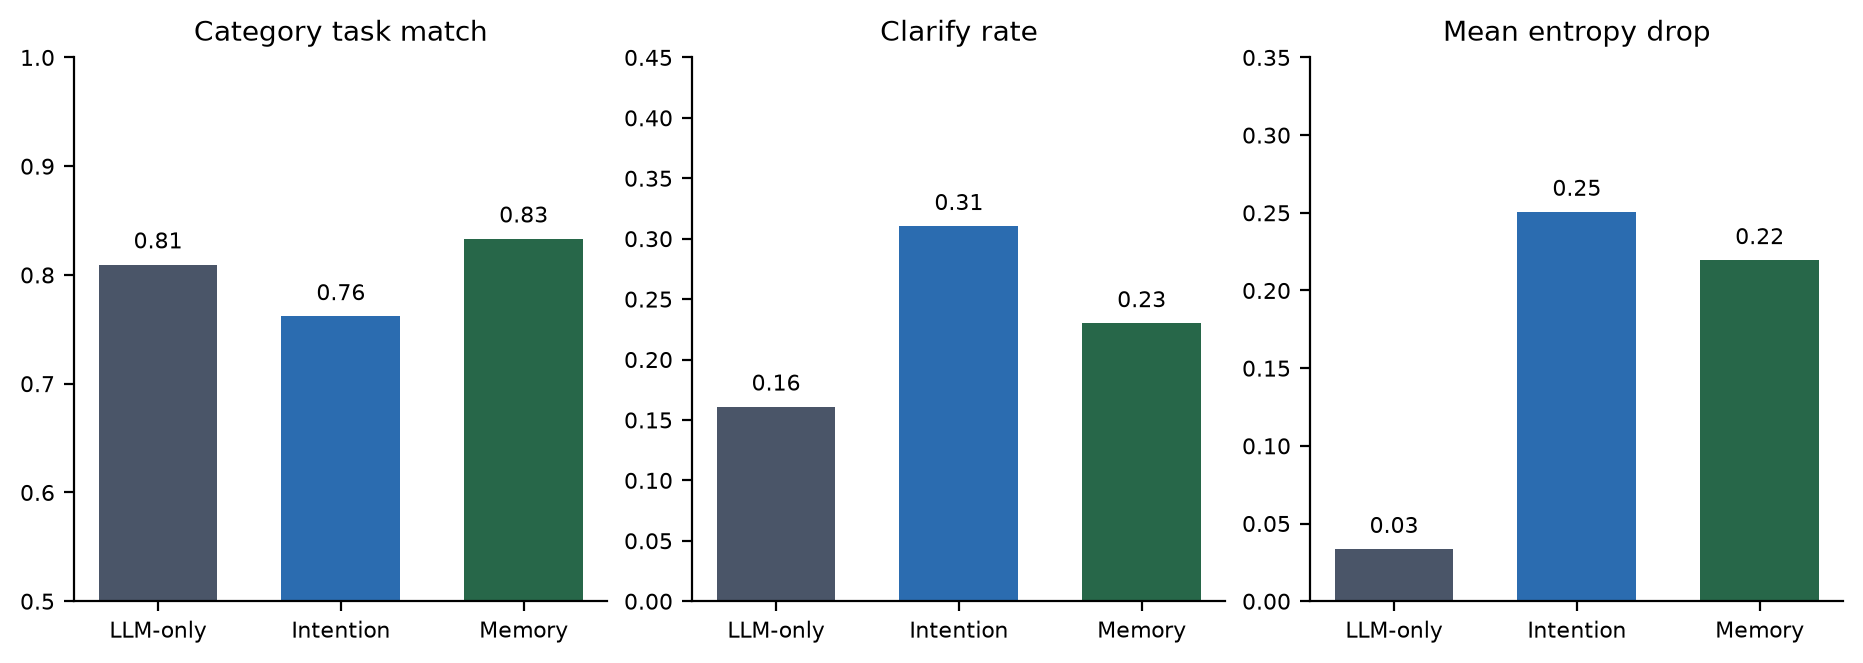
\includegraphics[width=0.96\textwidth]{figures/ch5_condition_contrasts.png}
  \caption{Selected scenario-level contrasts across the nested conditions ($N=42$):
  category task match, clarify rate, and mean entropy drop.}
  \label{fig:results-condition-contrasts}
\end{figure}

On aggregate, Memory-augmented attains the highest category match ($35/42$), LLM-only is next ($34/42$), and Intention-conditioned is slightly lower ($32/42$).
The privacy audit passes under all three conditions.
The largest separation among process measures is entropy drop and clarify rate: Intention-conditioned narrows belief most and clarifies most often, while LLM-only shows almost no entropy reduction on the logged path.

\section{Findings for RQ1}
\label{sec:results-rq1}

RQ1 contrasts LLM-only with Intention-conditioned on the same scenarios.
Category task match does not improve under Intention-conditioned operation: the rate falls from $0.810$ to $0.762$ (a net loss of two scenarios).
The sessions gained by Intention-conditioned relative to LLM-only are empty in this package; the two additional misses are boundary cases in which dining or travel wording overlaps wellness or fitness cues.

Process measures move in the opposite direction from match.
Mean entropy drop rises from $0.034$ to $0.251$, and the clarify rate nearly doubles ($0.161$ to $0.310$), with a corresponding decrease in suggest rate.
Resolution rate increases modestly ($0.619$ to $0.667$), while mean turns to resolution remain comparable.
Read locally, Intention-conditioned therefore buys inspectable belief narrowing and more frequent clarification under underspecification, without a concurrent gain in final category match on this package.

\section{Findings for RQ2}
\label{sec:results-rq2}

RQ2 contrasts Intention-conditioned with Memory-augmented, that is, the same intention-tracking path with and without the aggregate-memory prior.
Category task match rises from $0.762$ to $0.833$ (from $32/42$ to $35/42$).
The three recoveries are sessions in which a mild gold-aligned category prior corrects an otherwise unstable wellness or travel decision; they should be read as the effect of that controlled prior, not as proof of long-horizon user modelling.
Clarify rate falls from $0.310$ to $0.230$, and mean entropy drop remains substantial ($0.219$) though slightly below the Intention-conditioned value.

The prompt privacy audit remains perfect under Memory-augmented operation: raw identifiers and serialised detailed profiles do not enter the generative prompt.
For RQ2 as formulated in Section~\ref{sec:method-evaluation}, the privacy constraint is therefore satisfied on the reported items, while the behavioural gain is modest and prior-dependent.

\section{Error patterns}
\label{sec:results-errors}

Residual mismatches concentrate on class boundaries rather than on a single broken class.
Under Intention-conditioned operation, the ten misses are dominated by wellness--fitness swaps, beauty--medical skin wording, dining utterances pulled toward wellness, and travel openings that collide with fitness or medical cues.
Several of these sessions still emit clarify acts, so additional questioning does not reliably recover the gold category when lexical evidence remains thin.
LLM-only and Memory-augmented share many of the same boundary families; Memory-augmented removes only a subset of the Intention-conditioned misses, consistent with a mild category prior rather than a full repair of the extractor frontier.
